\documentclass[8pt,twocolumn]{article}

\usepackage[a4paper, margin=0.2in]{geometry}
\usepackage{titlesec}
\usepackage{enumitem}
\usepackage{amsmath}
\usepackage{hyperref}
\usepackage{graphicx}
\usepackage{tabularx}
\usepackage{xcolor}
\usepackage{setspace}
\usepackage{listings}  
\usepackage{dsfont}
\usepackage{amssymb}
\lstset{
  frame=tb,
  language=C,
  aboveskip=3mm,
  belowskip=3mm,
  showstringspaces=false,
  columns=flexible,
  basicstyle={\small\ttfamily},
  keywordstyle=\color{blue}\bfseries,       % <<<< keyword styling
  commentstyle=\color{gray}\itshape,
  stringstyle=\color{orange},
  numbers=none,
  breaklines=true,
  breakatwhitespace=true,
  tabsize=3,
  % If you want to highlight extra words:
  morekeywords={uint32_t,size_t,shmat,shmget, sem_t, sem_wait, sem_post, SharedMem} % add your own identifiers here
}

\setstretch{0.2}
\setlength{\extrarowheight}{0pt}
\setlength{\parskip}{0pt}
\begin{document}
\title{CS2106 Final Cheatsheet}
\author{@Wxy2003-xy}
\date{}
\maketitle
\begin{itemize}[leftmargin=2em]
    \setlength{\itemsep}{0pt} % No extra space between items
    \setlength{\parskip}{0pt}
    \item The child process from \texttt{fork()} receives a copy-on-write duplicate of the parent's memory and file descriptor table.
    \item Use \texttt{wait()} or \texttt{waitpid()} in the parent to reap the child and avoid zombie processes.
    \item Each child should call \texttt{exit()} (or return from \texttt{main()}) to terminate cleanly.
    \item \texttt{exec*()} functions replace the current process image with a new program. No return, no return back to the original prog
\end{itemize}
\begin{center}
\vspace{-1.0em}
\resizebox{\linewidth}{!}{
    \vspace{1.2em} % Small vertical gap between the two tables
    \begin{tabular}{|l|l|c|c|}
      \hline
      \textbf{Function} & \textbf{Arguments} & \textbf{PATH} & \textbf{CustEnv} \\
      \hline
      \texttt{execl(path, arg0, …, NULL)}    & Arg list, full path            & No  & No  \\
      \hline
      \texttt{execlp(file, arg0, …, NULL)}   & Arg list, search \texttt{PATH} & Yes & No  \\
      \hline
      \texttt{execle(path, arg0, …, NULL, envp)} & Arg list, full path        & No  & Yes \\
      \hline
      \texttt{execv(path, argv[])}           & Arg vector, full path         & No  & No  \\
      \hline
      \texttt{execvp(file, argv[])}          & Arg vector, search \texttt{PATH} & Yes & No  \\
      \hline
      \texttt{execvpe(file, argv[], envp[])} & Arg vector, \texttt{PATH}, env  & Yes & Yes \\
      \hline
      \end{tabular}
}
\vspace{-0.6em}
\end{center}
\begin{itemize}[leftmargin=2em]
    \setlength{\itemsep}{0pt} % No extra space between items
    \setlength{\parskip}{0pt}
    \item \texttt{int id=shmget(IPC\_PRIVATE, size, IPC\_CREAT|0600);}
    \item \texttt{alloc = (T*) shmat(id, NULL, 0);}
    \item \texttt{shmdt(alloc)}
    \item \texttt{shmctl(id, IPC\_RMID, 0);}
    \item \texttt{pthread\_create(\\ pthread\_t *thread, const pthread\_attr\_t *attr, void *(*start\_routine)(void *), void *arg)} \\
    Spawns a thread that shares the same address space. Returns \texttt{0} on success.  
    \item \texttt{pthread\_join(pthread\_t thread, void **retval)} \\
    Waits for a thread to finish and optionally retrieves its return value. Returns \texttt{0} on success.
    \item \texttt{pthread\_exit(void *retval)} \\
    Terminates the calling thread and makes \texttt{retval} available to \texttt{pthread\_join()}. Does not return.
    \item \texttt{sem\_init(sem, [0(thread)|1(process)], value)} — Initialize semaphore to given value.
    \item \texttt{sem\_wait(sem)} — Decrement; blocks if value is 0.
    \item \texttt{sem\_post(sem)} — Increment; unblocks one waiter if any.
    \item \texttt{sem\_destroy(sem)} — Cleans up; does not free memory.
    \item Used for mutual exclusion (binary semaphores) or limiting access (counting semaphores).
\end{itemize}
\vspace{-0.8em}
\textbf{Dining Philosophers: Limit-Seat Strategy}
\vspace{-0.6em}
\begin{itemize}
    \setlength{\itemsep}{0pt} % No extra space between items
    \setlength{\parskip}{0pt}
    \item Limits the number of philosophers who can attempt to pick up chopsticks to ensure progress.
    \item Prevents circular wait, breaking one of Coffman’s deadlock conditions.
    \item Starvation is still possible due to unfair scheduling.
\vspace{-0.6em}
\begin{lstlisting}
typedef struct {
    int _status[N];
    sem_t mutex;
    sem_t sem[N]; 
} SharedMem;
void takeChpStk(SharedMem* shm, int i) 
    sem_wait(&shm->mutex);
    shm->_status[i] = HUNGRY;
    safeToEat(shm, i);
    sem_post(&shm->mutex);
    sem_wait(&shm->sem[i]);            
void safeToEat(SharedMem* shm, int i) 
    if ((shm->_status[i] == HUNGRY) &&
        (shm->_status[LEFT] != EATING) &&
        (shm->_status[RIGHT] != EATING)) {
            shm->_status[i] = EATING;
            sem_post(&shm->sem[i]);} 
void putChpStk(SharedMem* shm, int i) 
    sem_wait(&shm->mutex);
    shm->_status[i] = THINKING;
    safeToEat(shm, LEFT);
    safeToEat(shm, RIGHT);
    sem_post(&shm->mutex);            
\end{lstlisting}
\vspace{-1.5em}
\end{itemize}
\textbf{Barrier turnstile}
\vspace{-0.6em}
\begin{lstlisting}[mathescape=true]
int *count;
sem_t *barrier, *mutex, *barrier2;

void init_barrier(int numproc) {
  sem_init(barrier, 1, 0);
  sem_init(barrier2, 1, 1);
  sem_init(mutex, 1, 1);
  *count = 0;
}
void reach_barrier() {
  sem_wait(mutex); //====================================$\downarrow$
  (*count)++;
  if (*count == nproc) {
    sem_wait(barrier2); // -----------------------------$\downarrow$
    sem_post(barrier);} // - - - - - - - - - - - - - - $\uparrow$
  sem_post(mutex); //====================================$\uparrow$

  sem_wait(barrier); // - - - - - - - - - - - - - - -$\downarrow$
  sem_post(barrier); // - - - - - - - - - - - - - - -$\uparrow$
  sem_wait(mutex); //====================================$\downarrow$
  (*count)--;
  if (*count == 0) {
    sem_wait(barrier); // - - - - - - - - - - - - - - -$\downarrow$
    sem_post(barrier2);} // ----------------------------$\uparrow$
  sem_post(mutex); //====================================$\uparrow$
  sem_wait(barrier2);   // -------------------------------$\downarrow$
  sem_post(barrier2);   // -------------------------------$\uparrow$
}
\end{lstlisting}
\begin{itemize}
    \setlength{\itemsep}{0pt} % No extra space between items
    \setlength{\parskip}{0pt}
    \item \textbf{Turnaround t}: Total time from job arrival to completion.
    \item \textbf{Response t}: Time from job arrival to first CPU execution.
    \item \textbf{Waiting time}: Time a job spends in the ready queue.
    \item \textbf{Throughput}: Number of jobs completed per unit time.
\end{itemize}
\vspace{-0.6em}
\resizebox{\linewidth}{!}{%
\begin{tabular}{|l|c|c|c|c|c|}
\hline
\textbf{Algorithm} & \textbf{Preemptive} & \textbf{Fairness} & \textbf{Resp T} & \textbf{Turarnd T} & \textbf{Starv} \\
\hline
FCFS    & No       & by order               & $\downarrow$                        & $\uparrow$ (convoy effect)       & $\downarrow$ \\
\hline
SJF     & No       & No                               & $\uparrow$ short jobs    & Optm (theo)      & $\uparrow$ \\
\hline
SRT     & Yes      & No                               & $\uparrow$ short jobs         & Optm                    & $\uparrow$ \\
\hline
RR      & Yes      & Yes                              & $\uparrow$                        & dep (qtm)& Low \\
\hline
Lottery & Can &                     & $\tilde{\text{Fair}}$             & $\tilde{\text{Fair}}$            & $\downarrow$ \\
\hline
MLFQ    & Yes      & Adaptive                         & $\uparrow$                   & Adaptive                   & dep \\
\hline
\end{tabular}%
}

\textbf{Table storage:}
\vspace*{-0.8em}
\begin{itemize}
    \setlength{\itemsep}{0pt} % No extra space between items
    \setlength{\parskip}{0pt}
    \item UPP: user process pages
    \item SWAP: Non-memory resident iser process page 
    \item Process page table: in PCB table in OS mem region in RAM
    \item Open file table: in OS mem region in RAM
    \item File descriptor table: in PCB 
    \item Dynamically allocated mem in a prgram: UPP or SWAP
    \item file decriptor returned from an open(...) syscall: UPP or SWAP
    \item compiled binary files: not part of the virtual mem
\end{itemize}
\vspace{-0.6em}
\textbf{Contiguous mem:}
\vspace{-0.6em}
\begin{itemize}
    \setlength{\itemsep}{0pt} % No extra space between items
    \setlength{\parskip}{0pt}
  \item \textbf{Tracking free space:}
\vspace{-0.6em}
  \begin{itemize}
    \setlength{\itemsep}{0pt} % No extra space between items
    \setlength{\parskip}{0pt}
    \item Bitmap: 1 bit per block, where 0 = free, 1 = allocated.
    \item Linked List: \texttt{<status, start\_idx, size, next*>}
    \item Buddy System: $2^n$ sized buddies: $ad_a$ XOR $ad_b$ = $2^n$
    \item \textbf{the rightmost bit is bit0, also the LSB}
  \end{itemize}
\vspace{-0.6em}
  \item \textbf{Fragmentation:}
\vspace{-0.6em}
  \begin{itemize}
    \setlength{\itemsep}{0pt} % No extra space between items
    \setlength{\parskip}{0pt}
    \item Internal (never in contiguous alloc if carve perfectly)
    \item External: Gaps between allocated blocks.
  \end{itemize}
\vspace{-0.6em}
\end{itemize}
\vspace{-0.6em}
\textbf{Paging}
\vspace{-0.6em}
\begin{itemize}
    \setlength{\itemsep}{0pt} % No extra space between items
    \setlength{\parskip}{0pt}
  \item Fixed-size units: Logical pages and physical frames.
  \item Page Table: Maps pages to frames.
  \item TLB: Hardware cache for recent page table entries.
\end{itemize}
\vspace{-0.6em}
\textbf{Segmentation}
\vspace{-0.6em}
\begin{itemize}
    \setlength{\itemsep}{0pt} % No extra space between items
    \setlength{\parskip}{0pt}
  \item Logical memory divided into named segments (text, data, stack, heap).
  \item Each has a base and limit.
  \item Logical Address = \texttt{<Segment\_ID, Offset>}.
  \item Different segments don't share page. As text and data can have different permissions
\end{itemize}
\vspace{-0.6em}
\textbf{Virtual mem}
\vspace{-0.6em}
\begin{itemize}
    \setlength{\itemsep}{0pt} % No extra space between items
    \setlength{\parskip}{0pt}
  \item Logical memory can exceed physical memory.
  \item $|\text{Virtual pages}|$ = $2^{\text{Virtual\_address bits}}$
\end{itemize}
\vspace{-0.6em}
\textbf{Demand Paging}
\vspace{-0.6em}
\begin{itemize}
    \setlength{\itemsep}{0pt} % No extra space between items
    \setlength{\parskip}{0pt}
  \item Pages are only loaded on access. No memory resident page 
  \item (+) Reduces startup time and memory usage.
  \item (-) more page fault at start; page fault can cascade on other processes (e.g. thrashing)
\end{itemize}
\vspace{-0.6em}
\textbf{Page Access}
\vspace{-0.6em}
\begin{lstlisting}
    Check page table:
        if memory resident: acess physical mem; done;
        else: [page fault] -> trap to OS
            locate page in secondary storage;
            load into physical mem;
            update page table;
            goto Check page table;
\end{lstlisting}
\vspace{-0.6em}
\[
\bar{T}_{access} = p_{TLB\_hit}(T_{TLB} + T_{RAM}) + (1 - p_{TLB\_hit}) \cdot\]
\[ \left[T_{RAM} + p_{page\_fault}T_{pf\_remedy} + (1 - p_{pf})T_{RAM}\right]\]
\vspace{-0.2em}
\textbf{Single-Level Direct paging}
\vspace{-0.6em}
\begin{itemize}
    \setlength{\itemsep}{0pt} % No extra space between items
    \setlength{\parskip}{0pt}
  \item Wasteful for sparse address spaces.
  \item page table size = $|page| \times$ \texttt{sizeof(entry)} 
\end{itemize}
\vspace{-0.6em}
\textbf{Multilevel}
\vspace{-0.6em}
\begin{itemize}
    \setlength{\itemsep}{0pt} % No extra space between items
    \setlength{\parskip}{0pt}
  \item Page directories point to page tables. dir size = page size
  \item max level: 
\vspace{-0.2em}
    \begin{enumerate}
      \setlength{\itemsep}{0pt} % No extra space between items
      \setlength{\parskip}{0pt}
      \item find branching factor \texttt{bf = page\_size / entry\_size}
      \item virtual address bits: \texttt{[(level $\times$ branching):ofst]}
      \item min mem for page table: \texttt{level $\times$ entry\_size}
      \item max: \texttt{[(level - 1) $\times$ frames + 1] $\times$ entry\_size}
    \end{enumerate}
\vspace{-0.2em}
  \item page dir base reg \texttt{$\rightarrow<$page\_dir\#, page\#, ofst$>$}
  \item overhead = \texttt{sizeof(page\_dir) + $\sum$sizeof(loaded leaf table)}
  \item min: clustered pages; max: sparse pages(more leaf tables loaded)
\end{itemize}
\vspace{-0.6em}
\textbf{Inverted Page Table}
\vspace{-0.6em}
\begin{itemize}
    \setlength{\itemsep}{0pt} % No extra space between items
    \setlength{\parskip}{0pt}
  \item One entry per frame: \texttt{<pid, page\#>} $\rightarrow$ frame.
  \item Compact but slow due to full-table lookup.
  \item page\# is not unique among processes
  \item pid + page\# can uniquely identify a memory page  
  \item (+) Efficient: One table for all processes;(-) Slow translation

\end{itemize}
\vspace{-0.6em}
\textbf{Temporal Locality:} Recently used memory will be used again.\\
\textbf{Spatial Locality:} Nearby memory addresses.\\
\textbf{Page Replacement Algorithms}
\vspace{-0.6em}
\begin{itemize}
    \setlength{\itemsep}{0pt} % No extra space between items
    \setlength{\parskip}{0pt}
    \item When a page is evicted
\vspace{-0.4em}
    \begin{itemize}
         \setlength{\itemsep}{0pt} % No extra space between items
    \setlength{\parskip}{0pt}
      \item Clean page: not modified $\rightarrow$ no need to write back
      \item Dirty page: modified $\rightarrow$ need to write back   
    \end{itemize}
\vspace{-0.4em}
  \item OPT: Replace page with furthest next use (ideal).
  \item FIFO: Oldest page out. (temporal locality $\rightarrow$ Belady's Anomaly: more frames, more page faults)
  \item LRU: Least recently used page.
  \item Clock: Approximate LRU using reference bits.
  \item \vspace{-0.6em} \begin{lstlisting}
// Modified FIFO to give a second chance to pages that are accessed
// Each PTE now maintains a "reference bit"
// 1 = Accessed, 0 = Not accessed
while (The oldest FIFO page is selected):
  If reference bit == 0  
    Page is replaced
  If reference bit == 1  
    Page is given a 2nd chance
    Reference bit cleared to 0
    Next FIFO page is selected
// When all pages have reference bit == 1
// Degenerates into FIFO algorithm
  \end{lstlisting}
\vspace{-0.6em}
\end{itemize}
\vspace{-1.0em}
\textbf{Frame allocation: N frames, M processes}
\vspace{-0.6em}
\begin{itemize}
  \setlength{\itemsep}{0pt} % No extra space between items
  \setlength{\parskip}{0pt}
  \item Equal alloc: Each process get N / M frames
  \item Proportional alloc: P gets $N\frac{\text{size}_P}{\sum \text{size}_{P_i}}$
\end{itemize}
\vspace{-0.8em}
\textbf{Local Replacement}
\vspace{-0.6em}
\begin{itemize}
    \setlength{\itemsep}{0pt} % No extra space between items
    \setlength{\parskip}{0pt}
  \item Only evict pages from the same process.
  \item Predictable and isolated.
  \item if not enf allocated, hinders process progress
\end{itemize}
\vspace{-0.6em}
\textbf{Global Replacement}
\vspace{-0.6em}
\begin{itemize}
    \setlength{\itemsep}{0pt} % No extra space between items
    \setlength{\parskip}{0pt}
  \item Victim page can belong to any process.
  \item More flexible, allows self-adjustment, but less stable.
  \item bad behaved process can affect others
\end{itemize}
\vspace{-0.6em}
\textbf{Thrashing}
\vspace{-0.6em}
\begin{itemize}
    \setlength{\itemsep}{0pt} % No extra space between items
    \setlength{\parskip}{0pt}
  \item Excessive page faults reduce CPU utilization.
  \item Can lead to cascading faults in global replacement.
  \item \textbf{Working Set Model:} Allocate enf frames for \texttt{W(t, $\Delta$)}.
\end{itemize}

\begin{itemize}
    \setlength{\itemsep}{0pt} % No extra space between items
    \setlength{\parskip}{0pt}
    \item A file is the smallest amount of information that can be written to secondary memory.
    It is a named collection of data, used for organizing secondary memory
    \item A file type is a description of the information contained in the file. A file extension is
    a part of the file name that follows a dot and identifies the file type
    \item \texttt{fork()} and \texttt{open($f$)} $\rightarrow$ \texttt{ref\_count$_{f}$++}
    \item \texttt{Close($f$)} $\rightarrow$ \texttt{ref\_count$_{f}$--}.
    \item Truncating a file means that all the information on the file is erased but the
    administrative entries remain in the file tables. Occasionally, the truncate operation
    removes the information from the file pointer to the end.
\end{itemize}
\begin{table}[h!]
    \centering
    \renewcommand{\arraystretch}{0.6}
    \begin{tabular}{|l|p{6cm}|}
    \hline
    \textbf{Aspect} & \textbf{Memory Management} \\
    \hline
    Underlying Storage & RAM \\
    \hline
    Access Speed & Constant \\
    \hline
    Unit of Addressing & Physical memory address \\
    \hline
    Usage & Address space for process \newline \textbf{Implicit} when process runs \\
    \hline
    Organization & \textbf{Paging/Segmentation}: determined by HW \& OS \\
    \hline
    \end{tabular}
    \end{table}

    \begin{table}[h!]
        \centering
        \renewcommand{\arraystretch}{0.6}
        \begin{tabular}{|l|p{6cm}|}
        \hline
        \textbf{Aspect} & \textbf{File System Management} \\
        \hline
        Underlying Storage & Disk \\
        \hline
        Access Speed & Variable disk I/O time \\
        \hline
        Unit of Addressing & Disk sector \\
        \hline
        Usage & Non-volatile data \newline \textbf{Explicit} access \\
        \hline
        Organization & \textbf{Many FS types}: ext* (Linux), FAT* (Windows), HFS* (Mac) \\
        \hline
        \end{tabular}
        \end{table}
        \vspace{-0.6em} % Small vertical gap between the two tables
\begin{itemize}
    \setlength{\itemsep}{0pt} % No extra space between items
    \setlength{\parskip}{0pt}
  \item \textbf{Protection}: [user, grp, others] \texttt{chmod 754} $\rightarrow$ \texttt{drwxr-xr--}
    \item A process uses the \texttt{open()} system call to access a file:
      \item Updates the process’s \textbf{Per-Process File Descriptor Table}: \texttt{fd} points to the corresponding system-wide table entry.
    \item Shared file descriptors:
\vspace{-0.6em}
    \begin{itemize}
        \setlength{\itemsep}{0pt} % No extra space between items
        \setlength{\parskip}{0pt}
      \item Two \texttt{fd}s pointing to the same system-wide entry share offset and metadata.
      \item Created using \texttt{dup/2()}, or inherited from \texttt{fork()}.
      \item Reading by one process advances the file offset, affecting the other process.
      \item call \texttt{open()} separately or \texttt{dup()} to not share ofst
    \end{itemize}
  \end{itemize}
  \begin{table}[ht]
    \centering
    \resizebox{\linewidth}{!}{
    \begin{tabular}{|l|c|c|c|c|}
    \hline
    \textbf{Feature} & \textbf{Contiguous} & \textbf{Linked List} & \textbf{FAT} & \textbf{Inode-based (e.g., ext)} \\
    \hline
    Access time (random) & Fast & Slow & Moderate & Fast \\
    Access time (sequential) & Fast & Fast & Fast & Fast \\
    Disk fragmentation & High & None & None & Low \\
    Supports random access & Yes & No & Yes (with FAT table) & Yes \\
    Space efficiency & Poor & Good & Good & Very good \\
    Pointer overhead & None & High & High (FAT in memory) & Low (indirect blocks) \\
    File size flexibility & Poor & Good & Good & Excellent \\
    Crash recovery & Poor & Poor & Moderate & Good (journaling) \\
    \hline
    \end{tabular}
    }
    \end{table}
\resizebox{\linewidth}{!}{
  \tiny
  \begin{tabular}{|l|c|c|}
  \hline
  \tiny
  \textbf{FAT12} & \textbf{FAT16} & \textbf{FAT32} \\
  \hline
  \tiny
  2$^{12}$ clusters  & 2$^{16}$ & 2$^{28}$ \\
  \hline
  \end{tabular}
}
\vspace{-0.6em}
\begin{itemize}
  \setlength{\itemsep}{0pt} % No extra space between items
  \setlength{\parskip}{0pt}
  \item \textbf{\texttt{open(const char *pathname, int flags[,mode])}}:
\vspace{-0.6em}
    \begin{itemize}
      \setlength{\itemsep}{0pt} % No extra space between items
      \setlength{\parskip}{0pt}
      \item Opens a file and returns a file descriptor (int).
      \item \texttt{flags}: \texttt{O\_RDONLY}, \texttt{O\_WRONLY}, \texttt{O\_RDWR}, \texttt{O\_CREAT}, etc.
      \item \texttt{mode} required if \texttt{O\_CREAT} is used, set permission bits.
    \end{itemize}
\vspace{-0.6em}
  \item \textbf{\texttt{read(int fd, void *buf, size\_t count)}}:
\vspace{-0.6em}
    \begin{itemize}
      \setlength{\itemsep}{0pt} % No extra space between items
      \setlength{\parskip}{0pt}
      \item Reads up to \texttt{count} bytes from \texttt{fd} into buffer \texttt{buf}.
      \item Returns the number of bytes read, or 0 on EOF.
      \item Advances the file offset by the number of bytes read.
    \end{itemize}
\vspace{-0.6em}
  \item \textbf{\texttt{write(int fd, const void *buf, size\_t count)}}:
\vspace{-0.6em}
    \begin{itemize}
      \setlength{\itemsep}{0pt} % No extra space between items
      \setlength{\parskip}{0pt}
      \item Writes up to \texttt{count} bytes from buffer \texttt{buf} to \texttt{fd}.
      \item Returns the number of bytes written.
      \item Advances the file offset by the number of bytes written.
    \end{itemize}
\vspace{-0.6em}
  \item \textbf{\texttt{lseek(int fd, off\_t offset, int whence)}}:
\vspace{-0.6em}
    \begin{itemize}
      \setlength{\itemsep}{0pt} % No extra space between items
      \setlength{\parskip}{0pt}
      \item Moves the file offset for \texttt{fd}.
      \item \texttt{whence} can be \texttt{SEEK\_SET}, \texttt{SEEK\_CUR}, or \texttt{SEEK\_END}.
    \end{itemize}
\vspace{-0.6em}
  \item \textbf{\texttt{close(int fd)}}:
\vspace{-0.6em}
    \begin{itemize}
      \setlength{\itemsep}{0pt} % No extra space between items
      \setlength{\parskip}{0pt}
      \item Closes \texttt{fd}.
      \item Releases the open file table entry.
    \end{itemize}
\vspace{-0.6em}
\end{itemize}
\vspace{-0.6em}
\textbf{File block allocation:}
\vspace{-0.6em}
\begin{itemize}
  \setlength{\itemsep}{0pt} % No extra space between items
  \setlength{\parskip}{0pt}
  \item Contiguous: (+) simple and fast; (-) ext.frag, files size need to be specified first
  \item Linkedlist: (+) no frag; (-) slow rand. access, extra mem usage for pointers, unreliable
  \item Linkedlist2: (+) faster (in mem traverse); (-) FAT keep tracks of all disk blocks in a partition, wasteful
  \item Indexed: IndexBlock[N] == N$^{th}$ Block address. (+) fast, Only index block of opened file needs to be in memory; (-) Limited maximum file size
\end{itemize}
\vspace{-0.6em}
\textbf{Directory structure:}
\vspace{-0.6em}
\begin{itemize}
  \setlength{\itemsep}{0pt} % No extra space between items
  \setlength{\parskip}{0pt}
  \item Linkedlist: Each entry represents a file; Store file name (minimum) and possibly other metadata; Store file information or pointer to file information  
  \item Hashtable: HashTable[K] is inspected to match file name. Usually chained collision resolution is used  
  \item File info: File information consists of: File name and other metadata; Disk blocks information  
\end{itemize}
\begin{itemize}
  \setlength{\itemsep}{0pt} % No extra space between items
  \setlength{\parskip}{0pt}
  \item EXT2 inode max file size: 
    \item $x_0$ direct, $x_1$ single-level indirect... $x_n$ n-level indir
    \item $t$ data block size, $p$ pointer size
    \item inode size: $p\sum_{i=0}^{n}x_i$
    \item max file size: $t\sum_{i=0}^{n}x_i(\frac{t}{p})^i$
\end{itemize}
\vspace{-0.6em}
\textbf{Open:}
\vspace{-0.6em}
\begin{lstlisting}
Process P opens file /.../.../.../F:
  Search system-wide table for existing entry E
    If found:
      Creates an entry in P's table to point to E
      Return a pointer to this entry 
    If not found, continue;
  Use full pathname to locate file F  
    If not found, open operation terminates with error
    When F is located:
      its file information is loaded into a new entry E in system-wide table;
      Creates an entry in P's table to point to E
      Return a pointer to this entry
// The returned pointer is used for further read/write operation
\end{lstlisting}
\begin{itemize}
  \setlength{\itemsep}{0pt} % No extra space between items
  \setlength{\parskip}{0pt}
  \item A = 1010, B = 1011, C = 1100, D = 1101, E = 1110
  \item 1 Kb = 1024 byte $\quad$ 1 Mb = $2^{20}$ byte $\quad$ 1 Gb = $2^{30}$ byte
  \item $2^8 = 256, 2^9 = 512, 2^{10} = 1024 = 1Kb, 2^{12} = 4096 = 4Kb$
  \item $2^{16} = 65,536 = 64Kb,\quad 2^{20} = 1,048,576 = 1Mb$
  \item $2^{32} = 4,294,967,296 = 4Gb$
\end{itemize}
\begin{itemize}
  \setlength{\itemsep}{0pt} % No extra space between items
  \setlength{\parskip}{0pt}
  \item Load and Save racing condition:
  \item $\forall I_i \rightarrow$ \{$I_{i, Load}, I_{i, Save}$\}
  \item All permutations of $\mathbb{I}$: \{$I_i | i \leq n$\}, \\ where $\forall I_i \in \mathbb{I}, I_{i, Load} \prec I_{i, Save} \land I_{i, Save} \prec I_{i+1, Load}$
\end{itemize}

\noindent\makebox[\columnwidth][c]{%
  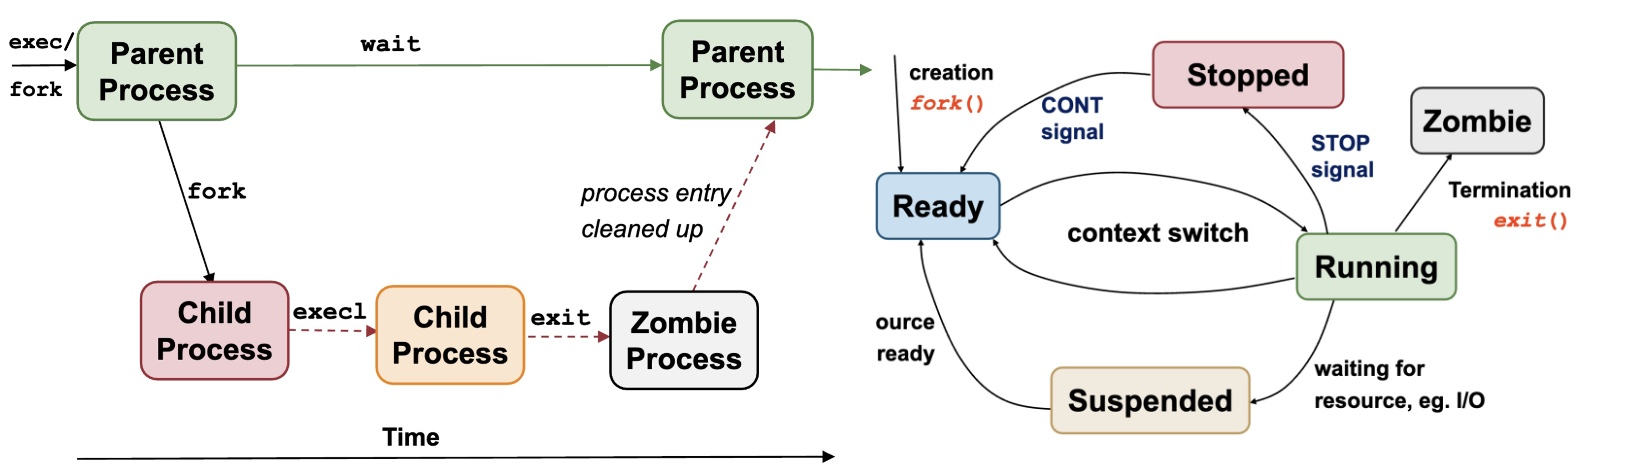
\includegraphics[
    width=\columnwidth,
    trim=0 0 0 0,
    clip
  ]{pro.jpg}%
}
\noindent\makebox[\columnwidth][c]{%
  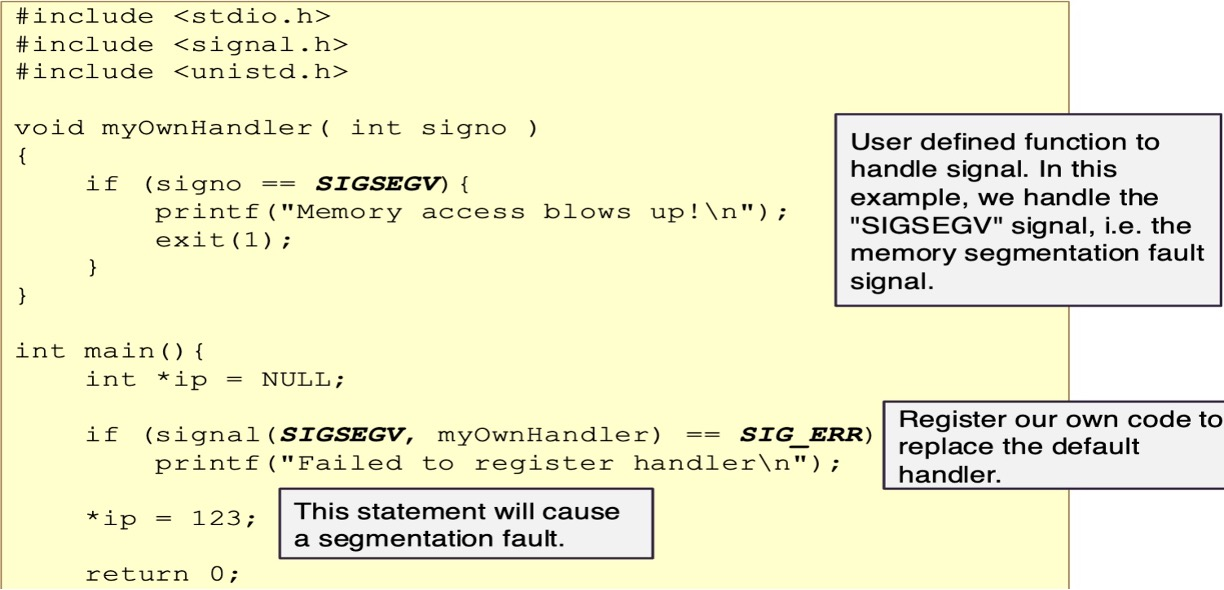
\includegraphics[
    width=\columnwidth,
    trim=0 0 0 0,
    clip
  ]{sig.jpg}%
}
\noindent\makebox[\columnwidth][c]{%
  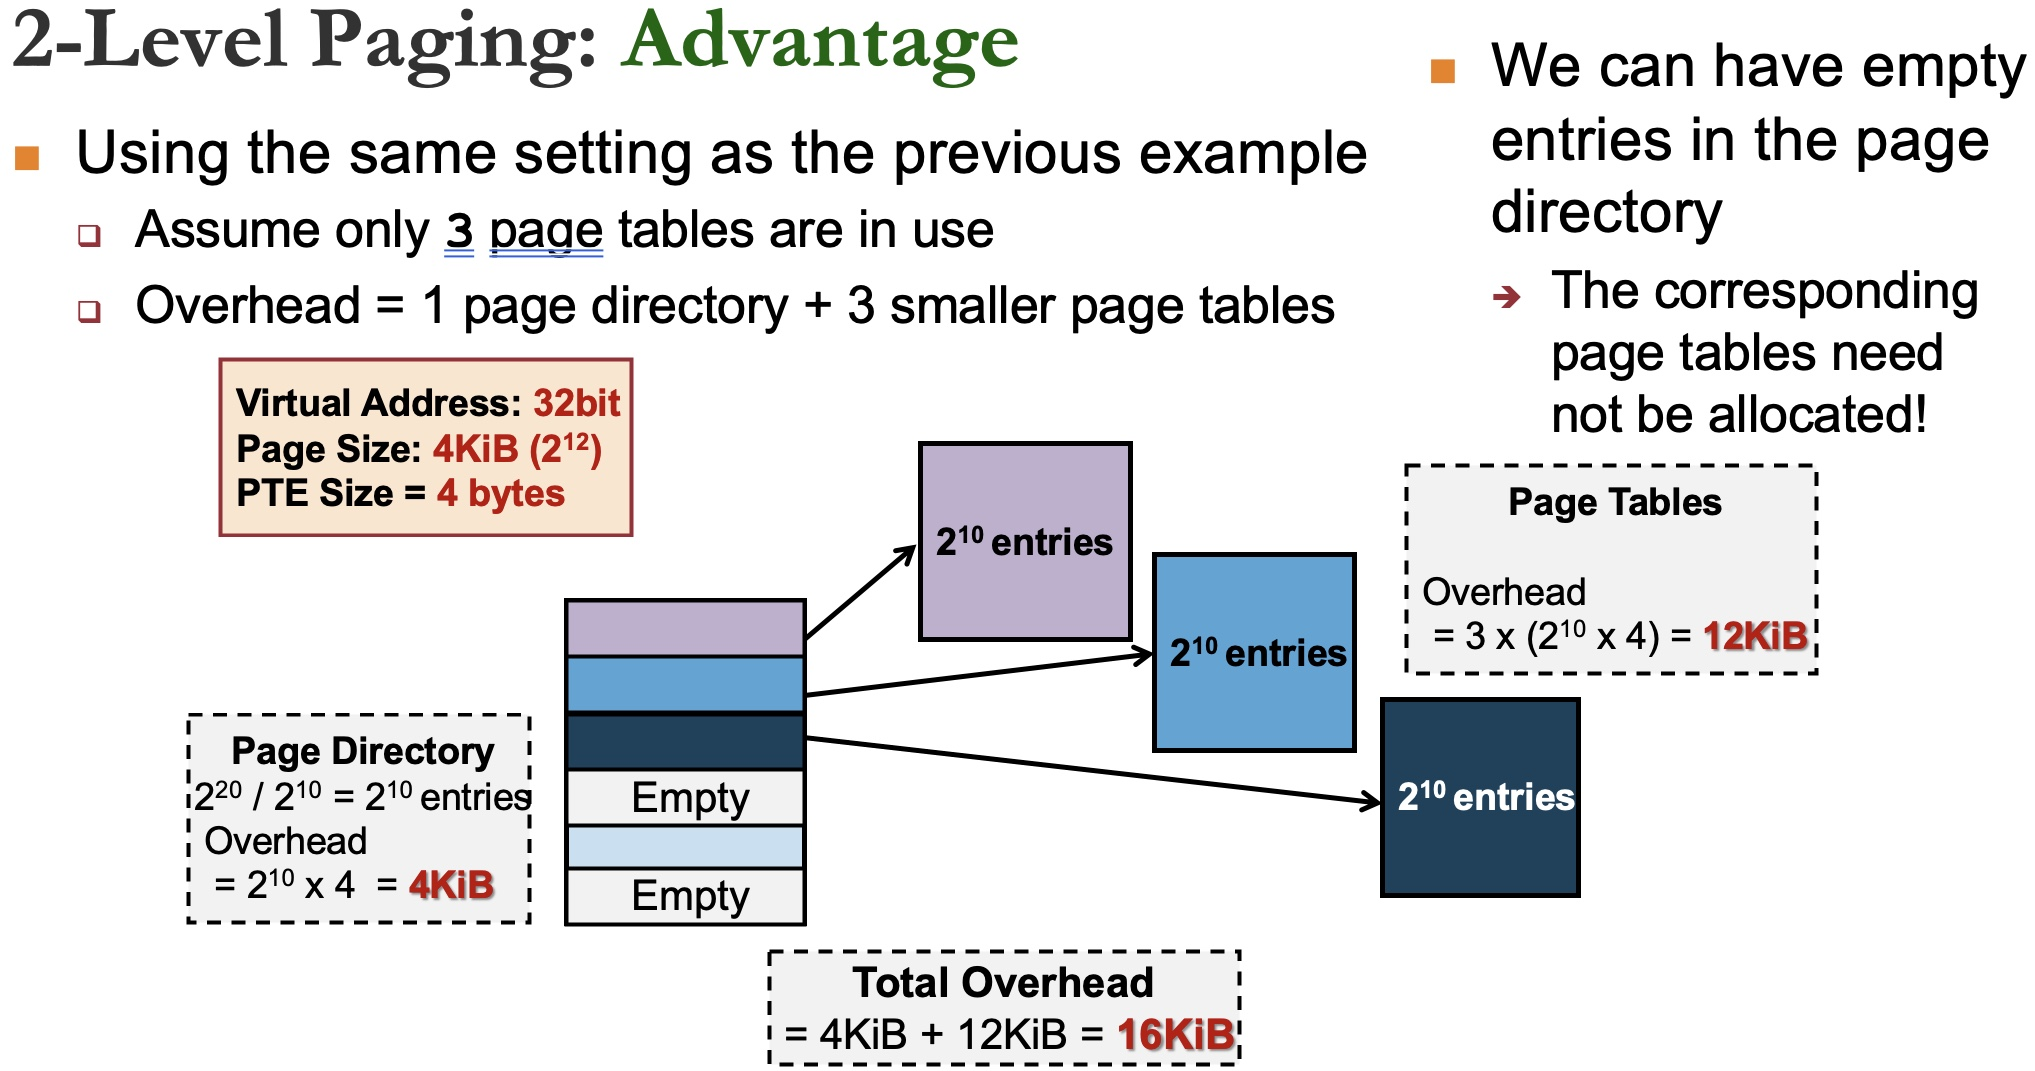
\includegraphics[
    width=\columnwidth,
    trim=0 0 0 0,
    clip
  ]{2lvl.jpg}%
}
\noindent\makebox[\columnwidth][c]{%
  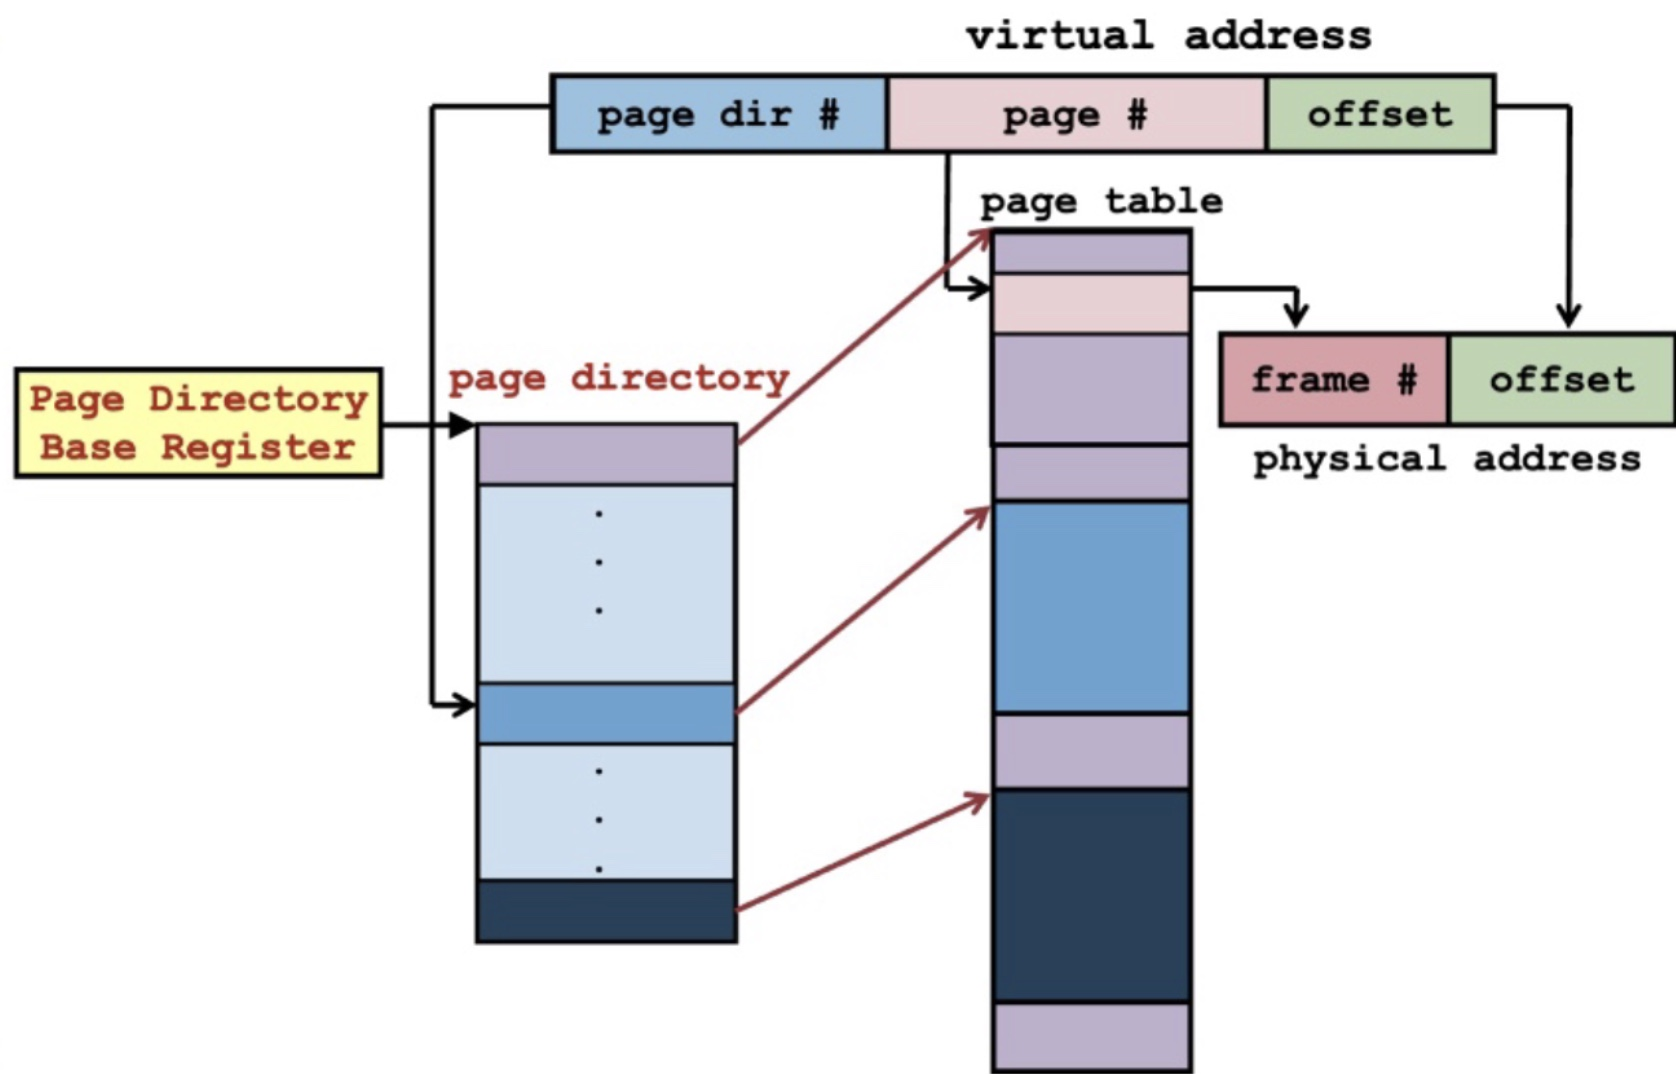
\includegraphics[
    width=\columnwidth,
    trim=0 0 0 0,
    clip
  ]{pgidx.jpg}%
}
\noindent\makebox[\columnwidth][c]{%
  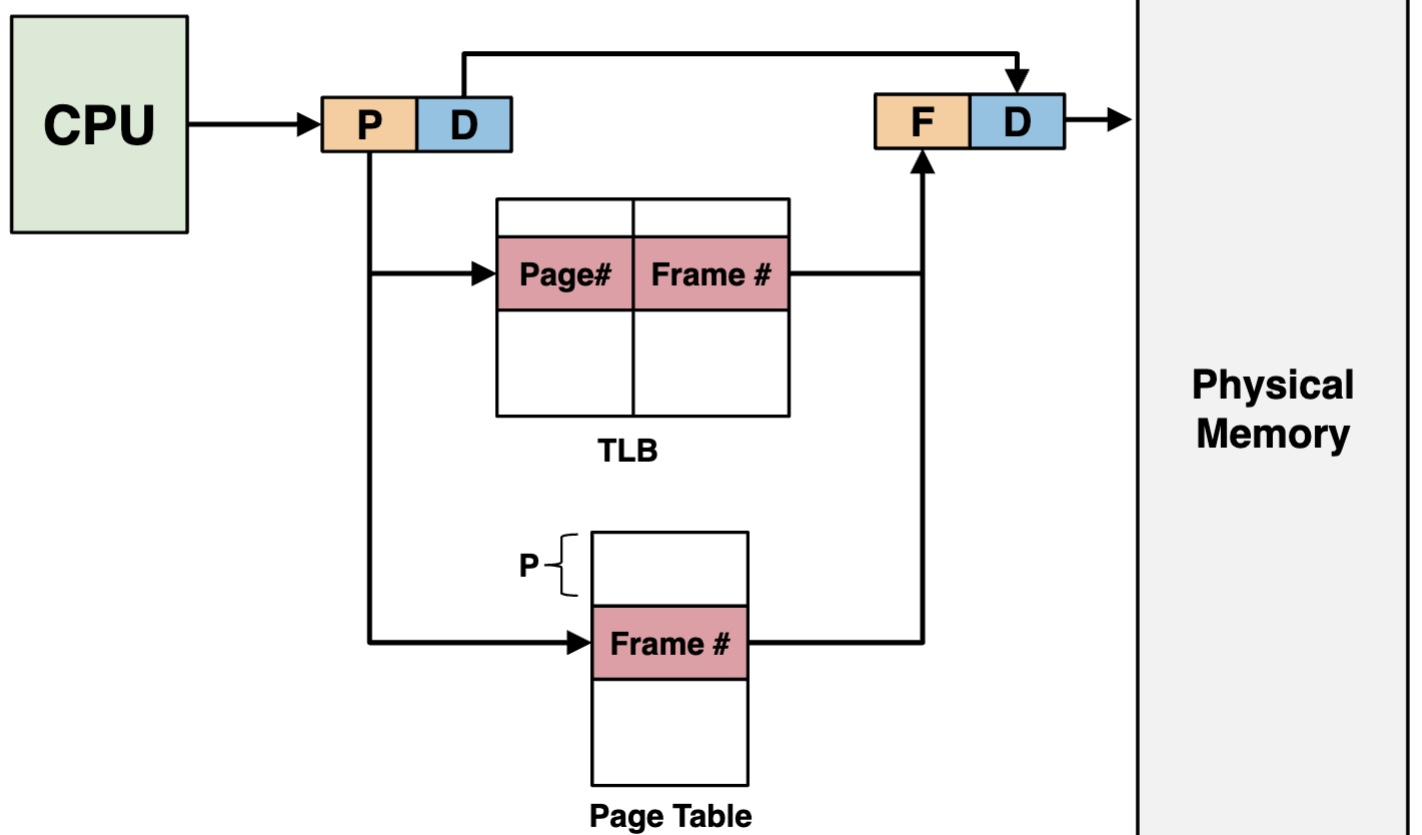
\includegraphics[
    width=\columnwidth,
    trim=0 0 0 0,
    clip
  ]{tlb.jpg}%
}
\noindent\makebox[\columnwidth][c]{%
  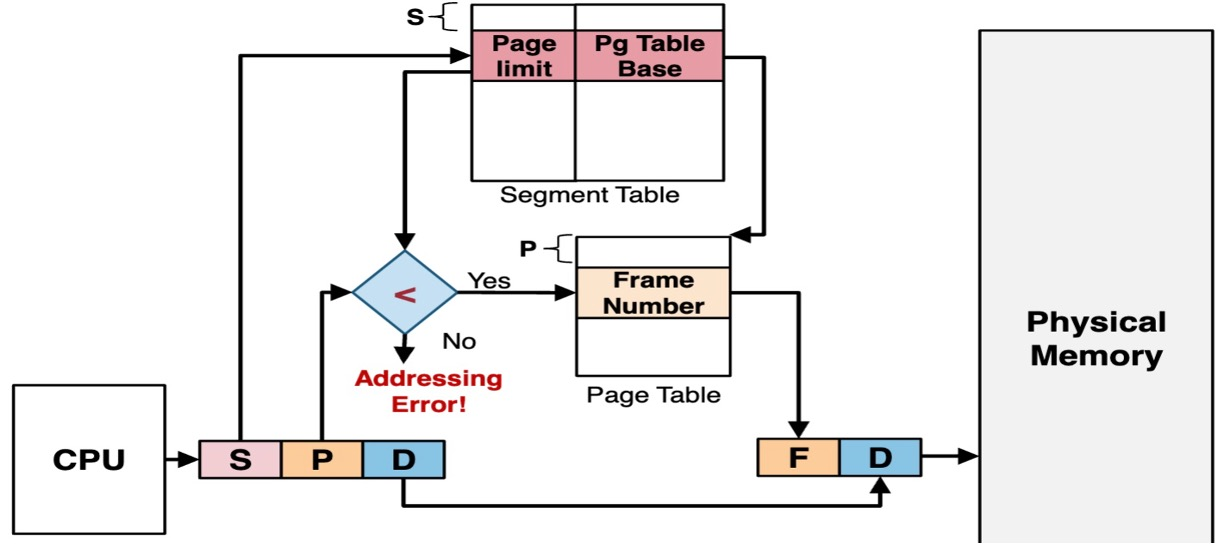
\includegraphics[
    width=\columnwidth,
    trim=0 0 0 0,
    clip
  ]{sgtb.jpg}%
}
\noindent\makebox[\columnwidth][c]{%
  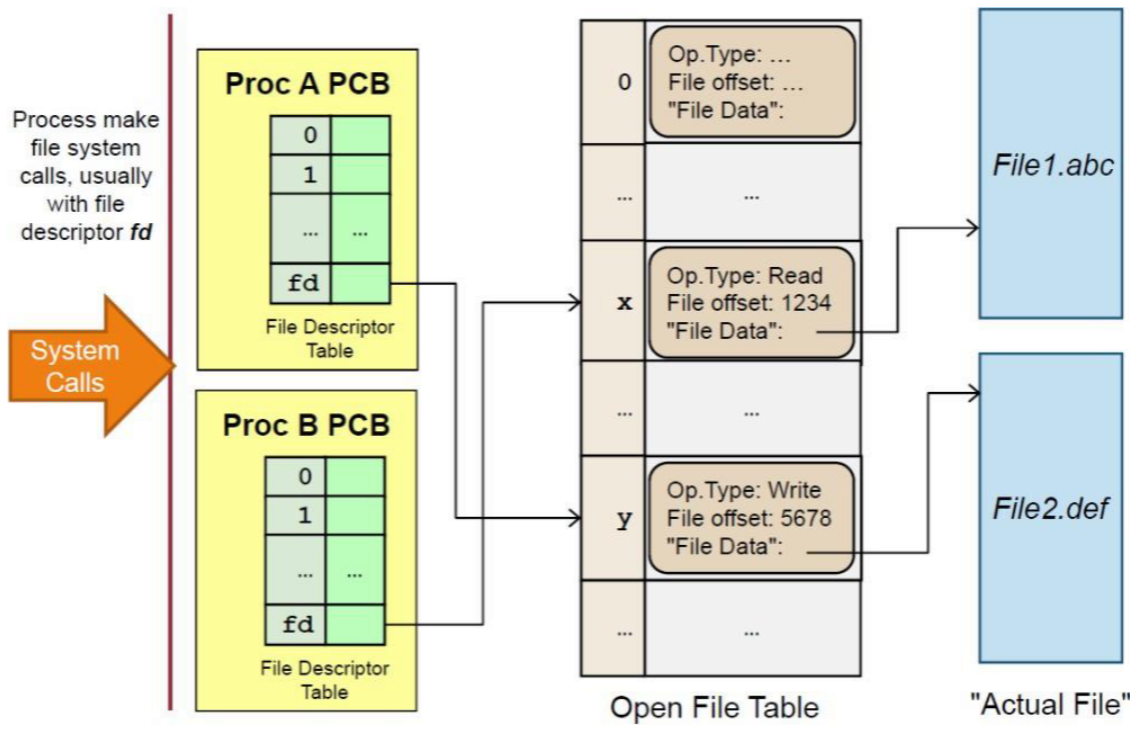
\includegraphics[
    width=\columnwidth,
    trim=0 0 0 0,
    clip
  ]{oft.png}%
}
\begin{itemize}
  \setlength{\itemsep}{0pt} % No extra space between items
  \setlength{\parskip}{0pt}\vspace{-0.6em}
  \item \textbf{System-wide Open-File Table}\vspace{-0.6em}
  \begin{itemize}
    \setlength{\itemsep}{0pt} % No extra space between items
    \setlength{\parskip}{0pt}
      \item One entry per unique file
  \end{itemize}\vspace{-0.6em}
  \item \textbf{Per-Process Open-File Table}\vspace{-0.6em}
  \begin{itemize}
    \setlength{\itemsep}{0pt} % No extra space between items
    \setlength{\parskip}{0pt}
      \item One entry per file used in the process
      \item Each entry points to the corresponding system-wide table entry
  \end{itemize}\vspace{-0.6em}
\end{itemize}\vspace{-0.6em}
\noindent\makebox[\columnwidth][c]{%
  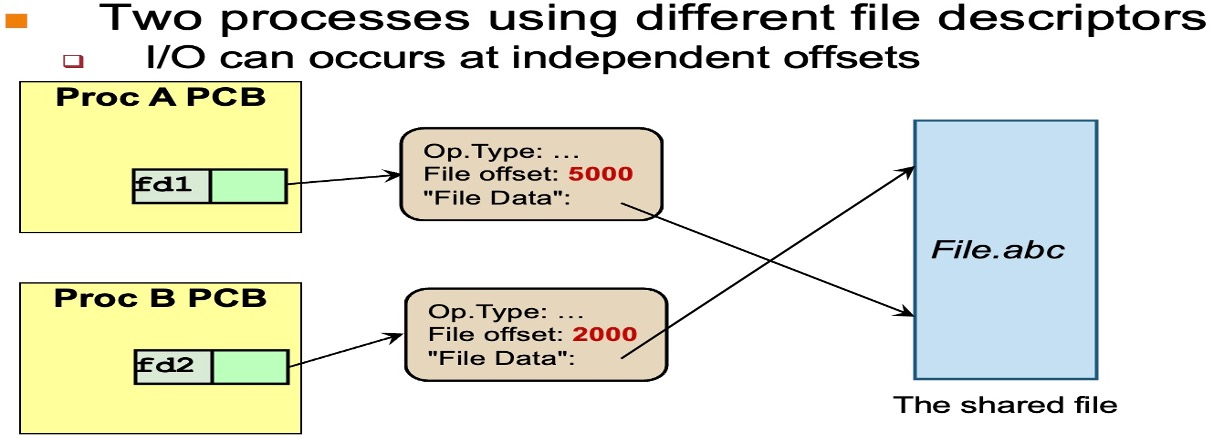
\includegraphics[
    width=\columnwidth,
    trim=0 0 0 0,
    clip
  ]{samefile2.jpg}
}
\noindent\makebox[\columnwidth][c]{%
  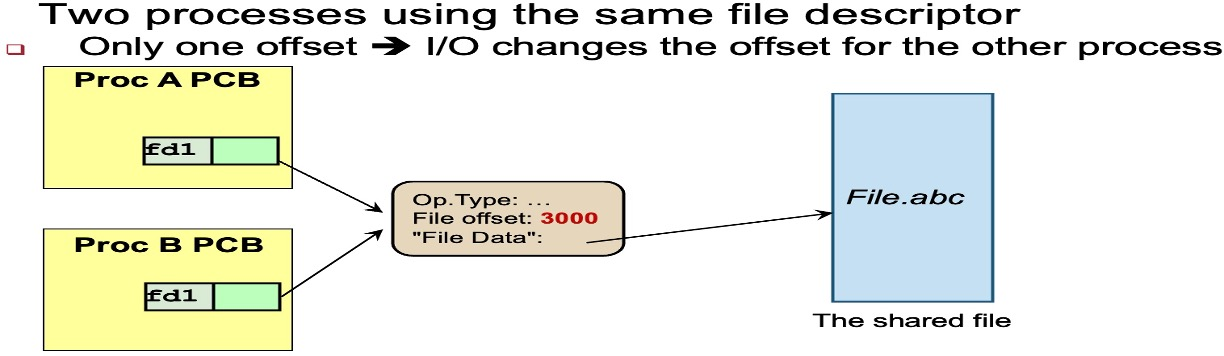
\includegraphics[
    width=\columnwidth,
    trim=0 0 0 0,
    clip
  ]{sameofst2.jpg}
}
\noindent\makebox[\columnwidth][c]{%
  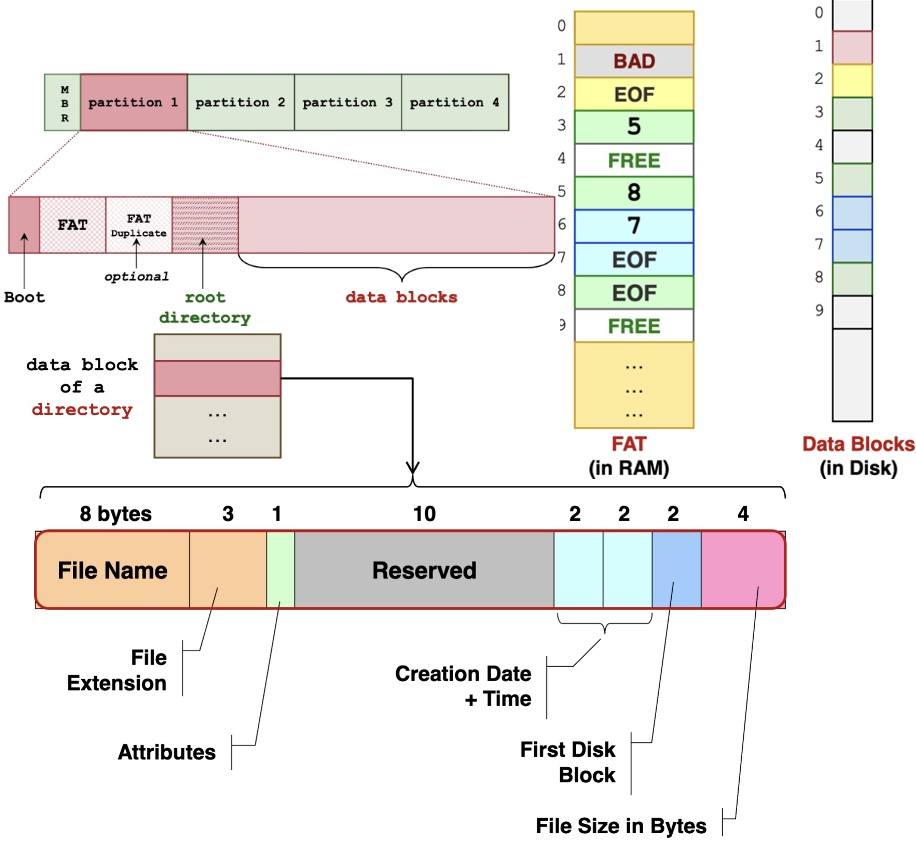
\includegraphics[
    width=\columnwidth,
    trim=0 0 0 0,
    clip
  ]{FAT.jpg}%
}
the actual size is a little lesser
Special values (EOF, FREE, etc.) reduces total number of valid data block/cluster indices
\noindent\makebox[\columnwidth][c]{%
  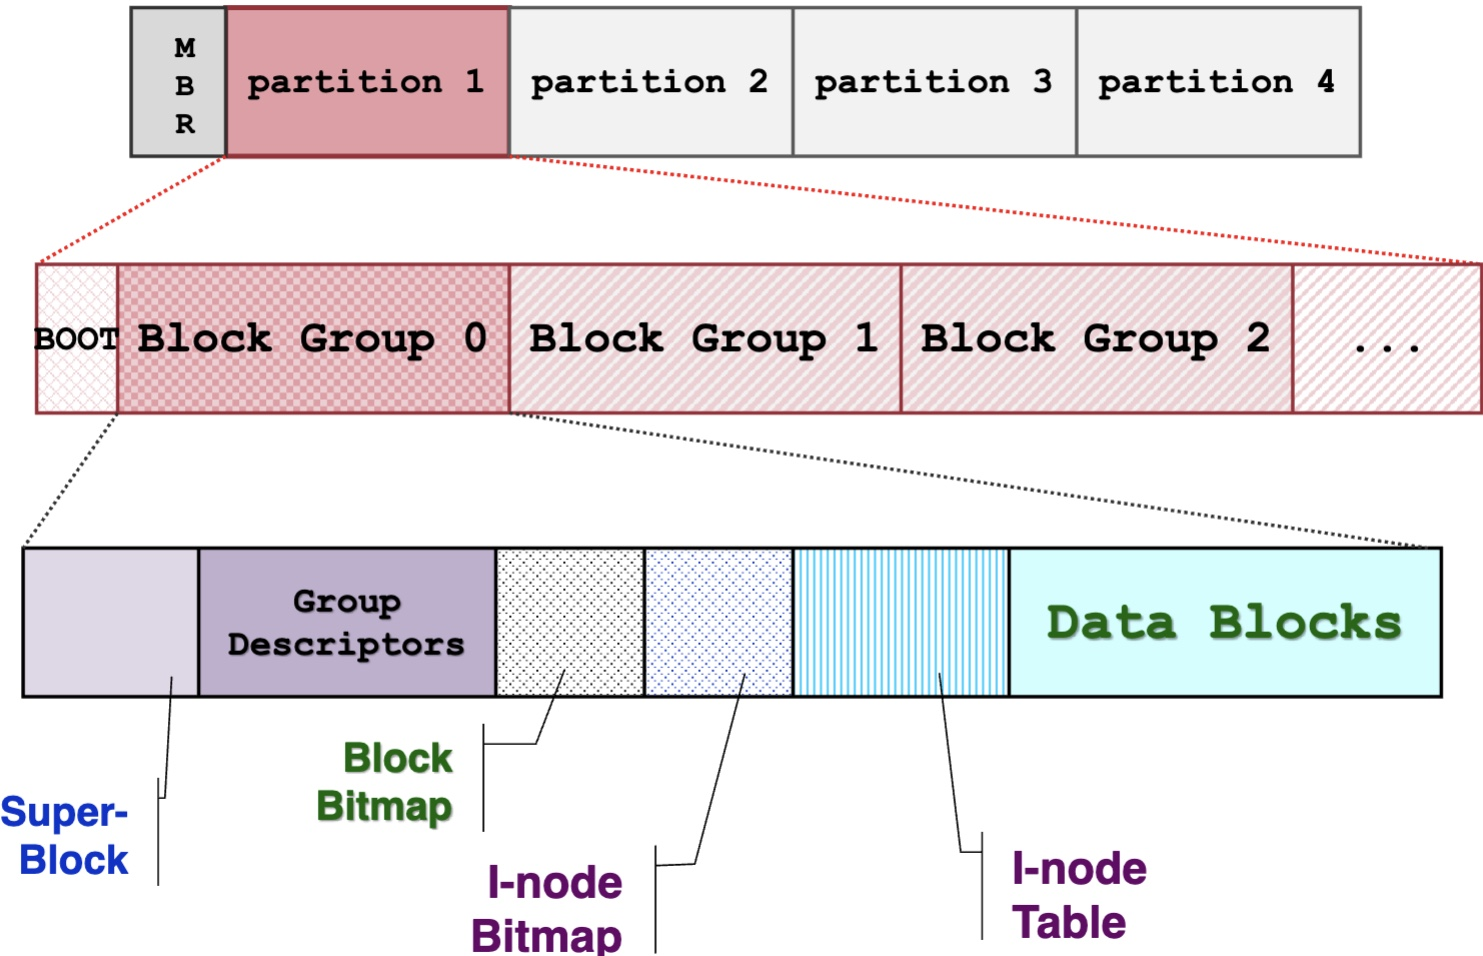
\includegraphics[
    width=\columnwidth,
    trim=0 0 0 0,
    clip
  ]{blkex.jpg}%
}
\vspace{-0.6em}
\begin{itemize}
  \small
  \setlength{\itemsep}{0pt} % No extra space between items
  \setlength{\parskip}{0pt}
  \item \textbf{Superblock}
\vspace{-0.6em}
  \begin{itemize}
    \setlength{\itemsep}{0pt} % No extra space between items
    \setlength{\parskip}{0pt}
      \item Describes the whole file system
      \item Includes:
      \begin{itemize}
        \setlength{\itemsep}{0pt} % No extra space between items
        \setlength{\parskip}{0pt}
          \item Total I-Nodes number, I-Nodes per group
          \item Total disk blocks, Disk Blocks per group
          \item etc.
      \end{itemize}
      \item Duplicated in each block group for redundancy
  \end{itemize}
\vspace{-0.6em}
  \item \textbf{Group Descriptors}
  \vspace{-0.6em}
  \begin{itemize}
    \setlength{\itemsep}{0pt} % No extra space between items
    \setlength{\parskip}{0pt}
      \item Describe each of the block groups
      \item Include:
      \begin{itemize}
        \setlength{\itemsep}{0pt} % No extra space between items
        \setlength{\parskip}{0pt}
          \item Number of free disk blocks, free I-Nodes
          \item Location of the bitmaps
      \end{itemize}
\vspace{-0.6em}
      \item Duplicated in each block group as well
  \end{itemize}
\end{itemize}
\vspace{-0.6em}
\begin{itemize}
  \setlength{\itemsep}{0pt} % No extra space between items
  \setlength{\parskip}{0pt}
  \item \textbf{Block Bitmap}
\vspace{-0.6em}
  \begin{itemize}
      \item Tracks the usage status of blocks in this block group
      \item 1 = Occupied, 0 = Free
  \end{itemize}
\vspace{-0.6em}
  \item \textbf{I-Node Bitmap}
\vspace{-0.6em}
  \begin{itemize}
    \setlength{\itemsep}{0pt} % No extra space between items
    \setlength{\parskip}{0pt}
      \item Tracks the usage status of I-Nodes in this block group
      \item 1 = Occupied, 0 = Free
  \end{itemize}
\vspace{-0.6em}
  \item \textbf{I-Node Table}
  \vspace{-0.6em}
  \begin{itemize}
    \setlength{\itemsep}{0pt} % No extra space between items
    \setlength{\parskip}{0pt}
      \item An array of I-Nodes
      \item Each I-Node is accessed by a unique index
      \item Contains only the I-Nodes of this block group
  \end{itemize}
\vspace{-0.6em}
\end{itemize}
\vspace{-0.6em}
\noindent\makebox[\columnwidth][c]{%
  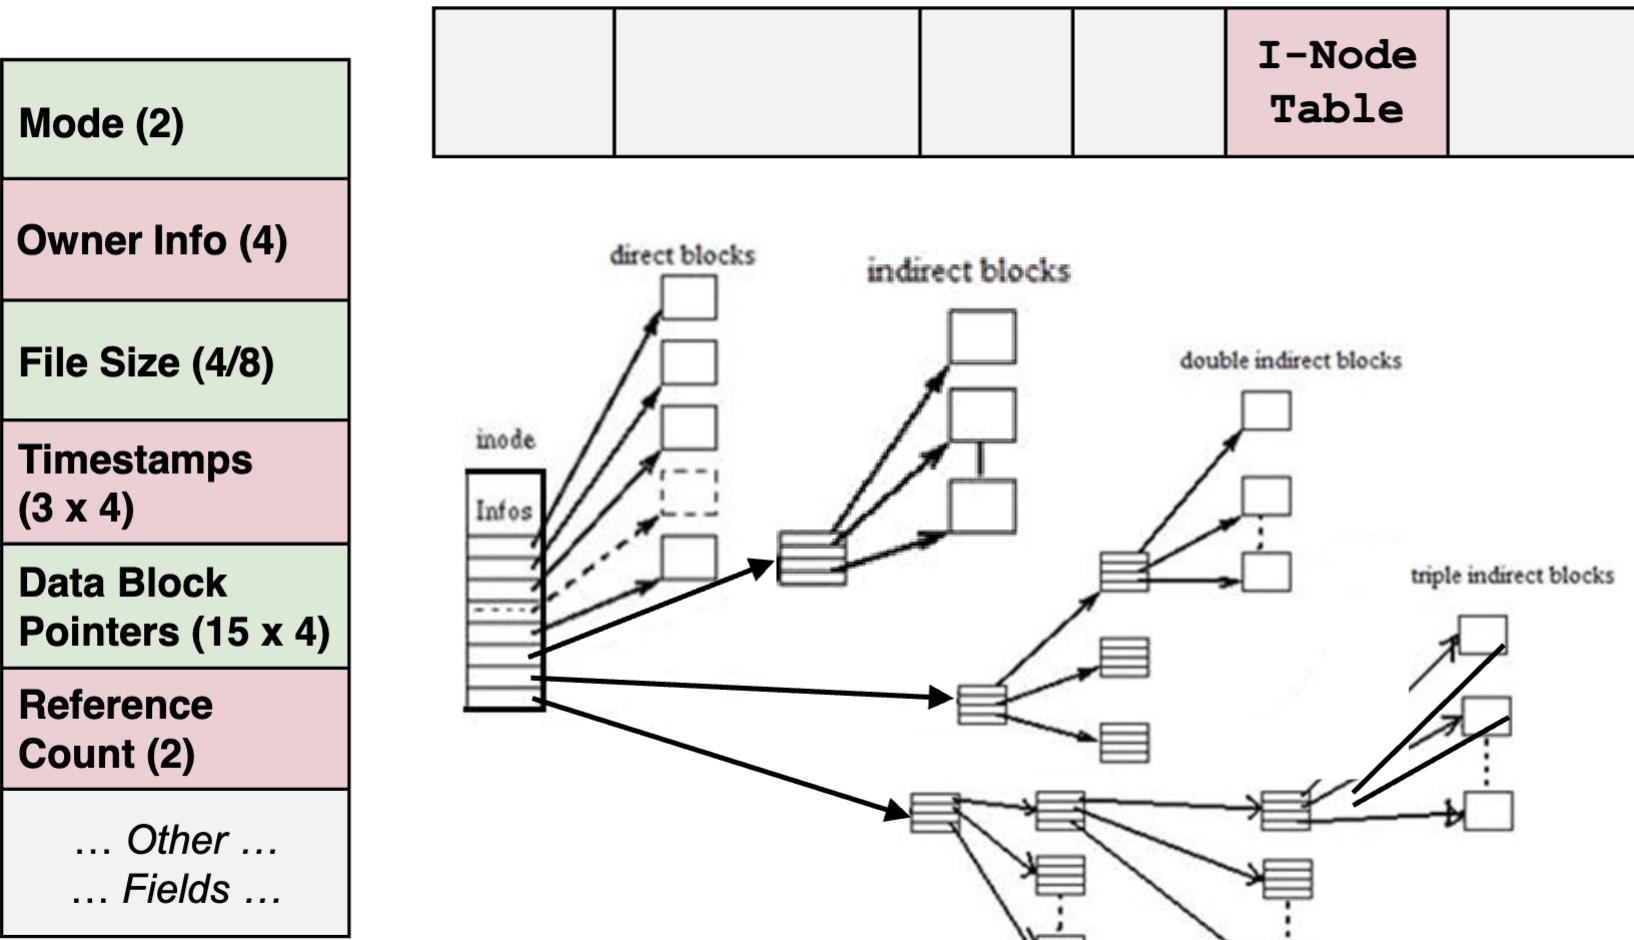
\includegraphics[
    width=\columnwidth,
    trim=0 0 0 0,
    clip
  ]{inode.jpg}%
}
\begin{itemize}
  \small
  \setlength{\itemsep}{0pt} % No extra space between items
  \setlength{\parskip}{0pt}
  \item \textbf{I-Node Contents}
\vspace{-0.6em}
\begin{itemize}
    \setlength{\itemsep}{0pt} % No extra space between items
    \setlength{\parskip}{0pt}
      \item Contains metadata for a file
      \item Contains 15 disk block pointers (disk block numbers)
  \end{itemize}
  \vspace{-0.6em}
  \item \textbf{Direct Blocks}
\vspace{-0.4em}
\begin{itemize}
    \setlength{\itemsep}{0pt} % No extra space between items
    \setlength{\parskip}{0pt}
      \item First 12 pointers
      \item Each points directly to a disk block containing actual data
  \end{itemize}
  \vspace{-0.6em}
  \item \textbf{Single Indirect Block}
\vspace{-0.4em}
\begin{itemize}
    \setlength{\itemsep}{0pt} % No extra space between items
    \setlength{\parskip}{0pt}
      \item 13th pointer
      \item Points to a disk block containing a list of direct block pointers
  \end{itemize}
  \vspace{-0.6em}
  \item \textbf{Double Indirect Block}
\vspace{-0.4em}
\begin{itemize}
    \setlength{\itemsep}{0pt} % No extra space between items
    \setlength{\parskip}{0pt}
      \item 14th pointer
      \item Points to a disk block that contains single indirect block pointers
  \end{itemize}
  \vspace{-0.6em}
\end{itemize}
\vspace{-1.2em}
\begin{itemize}
  \small
  \setlength{\itemsep}{0pt} % No extra space between items
  \setlength{\parskip}{0pt}
  \item \textbf{Directory Data Blocks}\vspace{-0.6em}
  \begin{itemize}
    \setlength{\itemsep}{0pt} % No extra space between items
    \setlength{\parskip}{0pt}
      \item Store a linked list of directory entries
      \item Each entry holds metadata for files or subdirectories contained in the directory
  \end{itemize}
  \vspace{-0.6em}
  \item \textbf{Each Directory Entry Contains:}\vspace{-0.6em}
  \begin{itemize}
    \setlength{\itemsep}{0pt} % No extra space between items
    \setlength{\parskip}{0pt}
      \item I-Node number for the file or subdirectory
      \item Size of this directory entry (to locate the next entry)
      \item Length of the file/subdirectory name
      \item Type: File or Subdirectory
      \item May also indicate other special file types
      \item File/Subdirectory name (up to 255 characters)
  \end{itemize}\vspace{-0.6em}
\end{itemize}
\noindent\makebox[\columnwidth][c]{%
  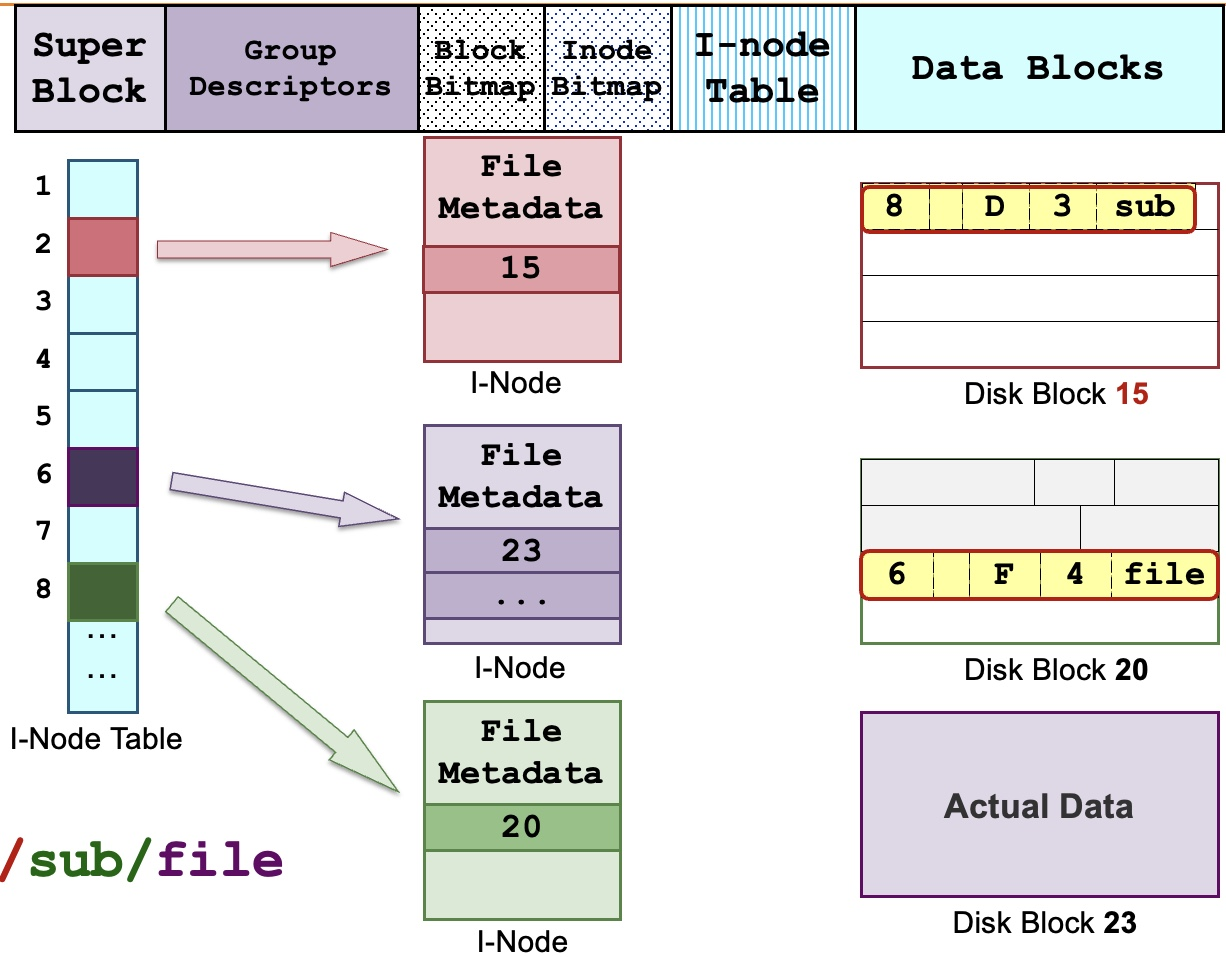
\includegraphics[
    width=\columnwidth,
    trim=0 0 0 0,
    clip
  ]{ext2ind.jpg}
}
\vspace{-0.6em}
\begin{itemize}
  \small
  \setlength{\itemsep}{0pt} % No extra space between items
  \setlength{\parskip}{0pt}
  \vspace{-0.6em}
  \item \textbf{Hard Link Problems}
  \vspace{-0.4em}
  \begin{itemize}
    \setlength{\itemsep}{0pt} % No extra space between items
    \setlength{\parskip}{0pt}
      \item Multiple references to the same I-Node make deletion management difficult
      \item Requires maintaining an I-Node reference count
      \item The reference count is decremented on each deletion
  \end{itemize}
  \vspace{-0.4em}
  \item \textbf{Symbolic Link Problems}\vspace{-0.4em}
  \begin{itemize}
    \setlength{\itemsep}{0pt} % No extra space between items
    \setlength{\parskip}{0pt}
      \item Stores only the pathname of the target file
      \item Can be easily invalidated due to:
      \begin{itemize}
        \setlength{\itemsep}{0pt} % No extra space between items
        \setlength{\parskip}{0pt}
          \item File name changes
          \item File deletions
      \end{itemize}
      \vspace{-0.4em}
      \item Requires a path lookup to resolve the actual I-Node of the target file
      \item Behaves like a normal file opening operation
  \end{itemize}\vspace{-0.6em}
\end{itemize}
\vspace{-0.6em}
\noindent\makebox[\columnwidth][c]{%
  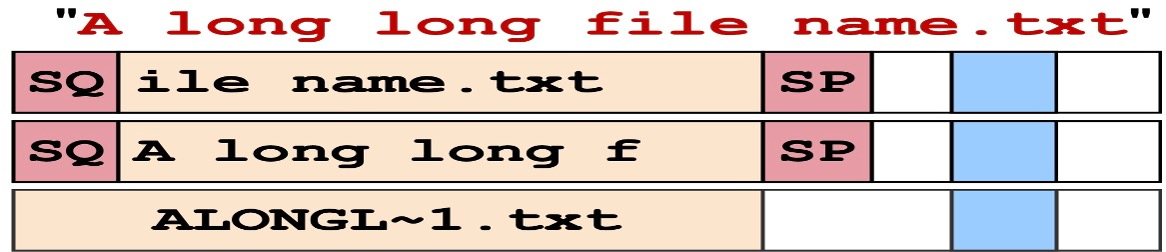
\includegraphics[
    width=\columnwidth,
    trim=0 0 0 0,
    clip
  ]{lnm.jpg}
}
Use multiple directory entries for a file with long file name; 
Need to keep the 8+3 short version for backward compatibility
\noindent\makebox[\columnwidth][c]{%
  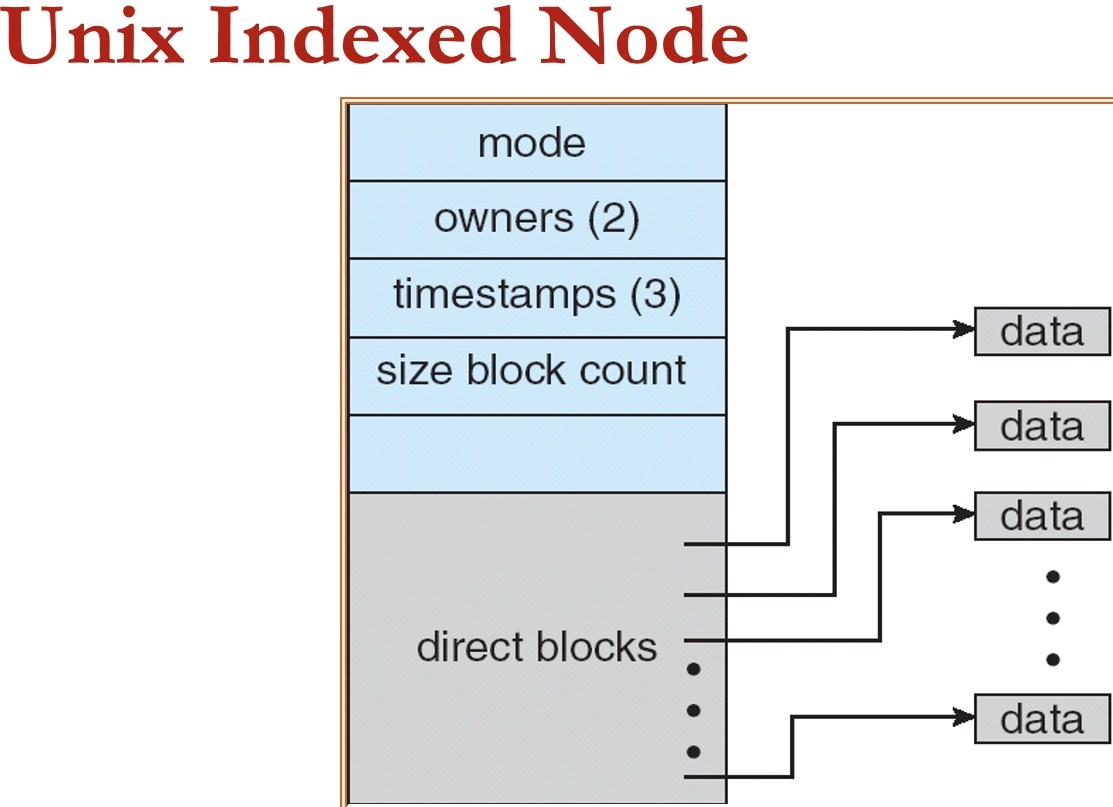
\includegraphics[
    width=\columnwidth,
    trim=0 0 0 0,
    clip
  ]{idxnode.jpg}
}

\end{document}
